\documentclass[a4paper]{ctexart}
\usepackage{amsmath}
\usepackage{indentfirst}

\ctexset{
section = {
format = \raggedright\large\bfseries,
}
}

\pagestyle{plain}	% 取消页眉

\title{Modern Ship Construction Technology}
\author{XinyuJian\\515021910260}


\begin{document}
\maketitle
\section{Introduction}
This little app is developed by XinyuJian. Its basic function is to plot the points and fair the curves.\\ 
The development environment is PyCharm+Anaconda. \\
The packages and their versions that it includes are as followings:\\
\begin{enumerate}
	\item numpy 1.14.3
	\item scipy 1.0.0
	\item wxPython 4.0.1
\end{enumerate}
Specifically, I used wxGlade, which is a GUI tool of wxPython, to simplify the development process.

\section{Mathematic Kernal}
The curve is actually a cubic spline with the following expresion. 
\begin{equation}
	y=a_0 a_1x+a_2x^2+a_3x^3+\sum_{i=2}^{n-1}a_{i+2}(x-x_i)^3
\end{equation}
The main idea is that using the least suqares method to fair the curve, which is the solution of the next expression:
\begin{equation}
	\min_{b}||Ab-Y||_2, A\in C^{n\times m}, Y\in C^{n}
\end{equation}
The special solution is the product of the generalized inverse matrix of $A$ and $Y$, which is also the solution of the minimal norm. The general solution is the special solution plus the zero space of $A$. Here, we omit the derivative process.
\section{Structure Tree}
There are four main files.\\
\begin{enumerate}
	\item $curve-fitting.py$: Main body of the app. Integrate the functionalities and provide the application program interface.
	\item $curve-fitting-GUI.py$: Provide GUI source code and provide the application program interface to $curve-fitting.py$, generated by wxGlade.
	\item $matplotlib-canvas$: The outside function to plot, fit curve and fairing curve.
	\item $curve-fitting-GUI.wxg$: The wxGlade file.
\end{enumerate}

\section{Usage}
\subsection{Start}
You can run the app simply by double clicking the $curve-fitting.exe$ in Windows or running $curve-fitting.py$ in a python IDE. However, there is a problem if you choose first method. You will receive a warning saying that a $.jpg$ file cannot be found. The reason is that I put a school-logo at upper-left corner of the user interface and after conveying the project to an excutable file, the picture's direction has lost. For now, I have no way to deal with that. Please contact me if you have any solution. And in the second starting way, you may change the Line 43 in $curve-fitting-GUI.py$ in your directory of the logo.
\subsection{Interaction}
When you start the app, the user interface should look like Fig.\ref{fig}:
\begin{figure}[!htbp]
	\centering
	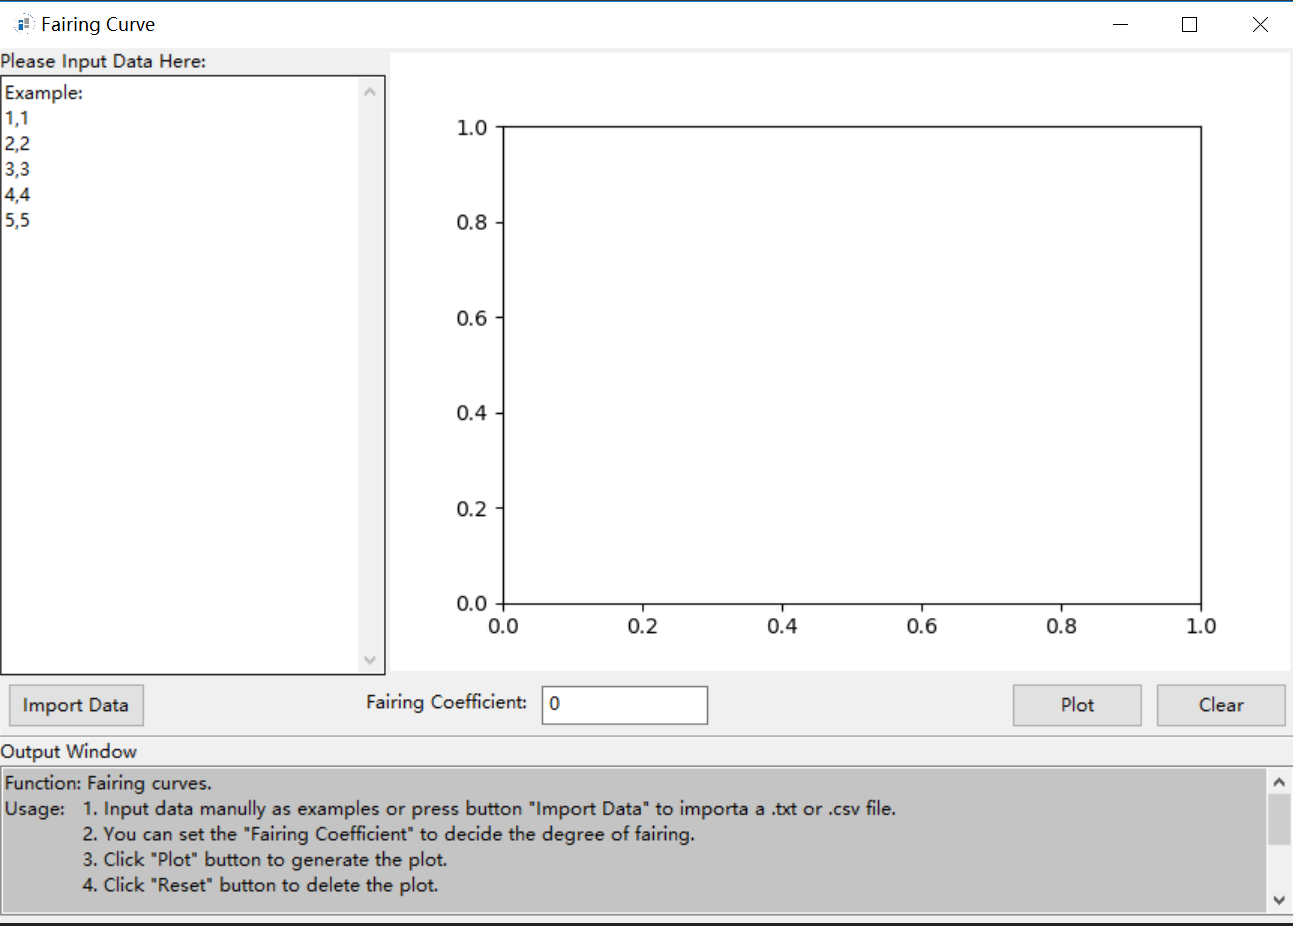
\includegraphics[width=4in]{interface}
	\caption{User Interface}
	\label{fig}
\end{figure}
The upper left is the place that you can input the data manually. The data structure should be the same as the example. Caution: delete example before your inputting. Note: There are two types of input data. One is that without weight, just like the example. One is that with weight, please refer Fig.\ref{weighted}.\\
The upper right is the section that a plot shows.\\
When you click the button "Import data", you can select a $.txt$ file or $.csv$ file to import data automatically. Be sure that the format is the same as the upper left. When it finished, the data will show in the upper left dialog window and the output window will show its direction. If the data structure were wrong, you will receive a warning in the output window. \\
You can specifiy the fairing coefficient to decide the degree of fairing. Generally, the bigger number means a better result.\\
When you click the button "Plot" after importing data, a plot will show in the upper right window.\\
When you click the button "Reset", the plot will be deleted.\\
As you can see, an output window is in the bottom. There will be a brief introduction by default.\\
Here are two examples.
\begin{figure}[!htbp]
	\centering
	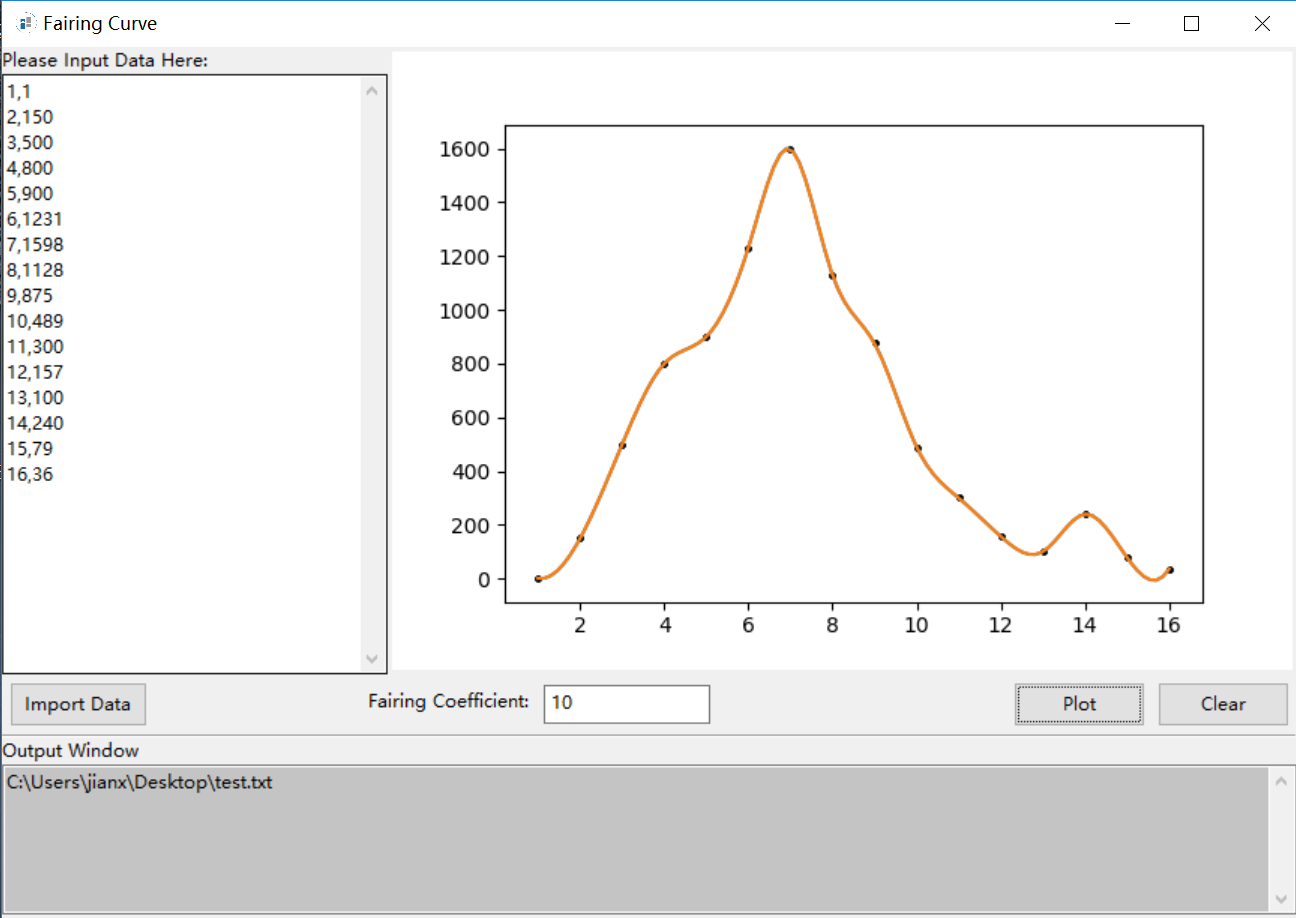
\includegraphics[width=4in]{example}
	\caption{An example without weight}
	\label{fige}
\end{figure}
\begin{figure}[!htbp]
	\centering
	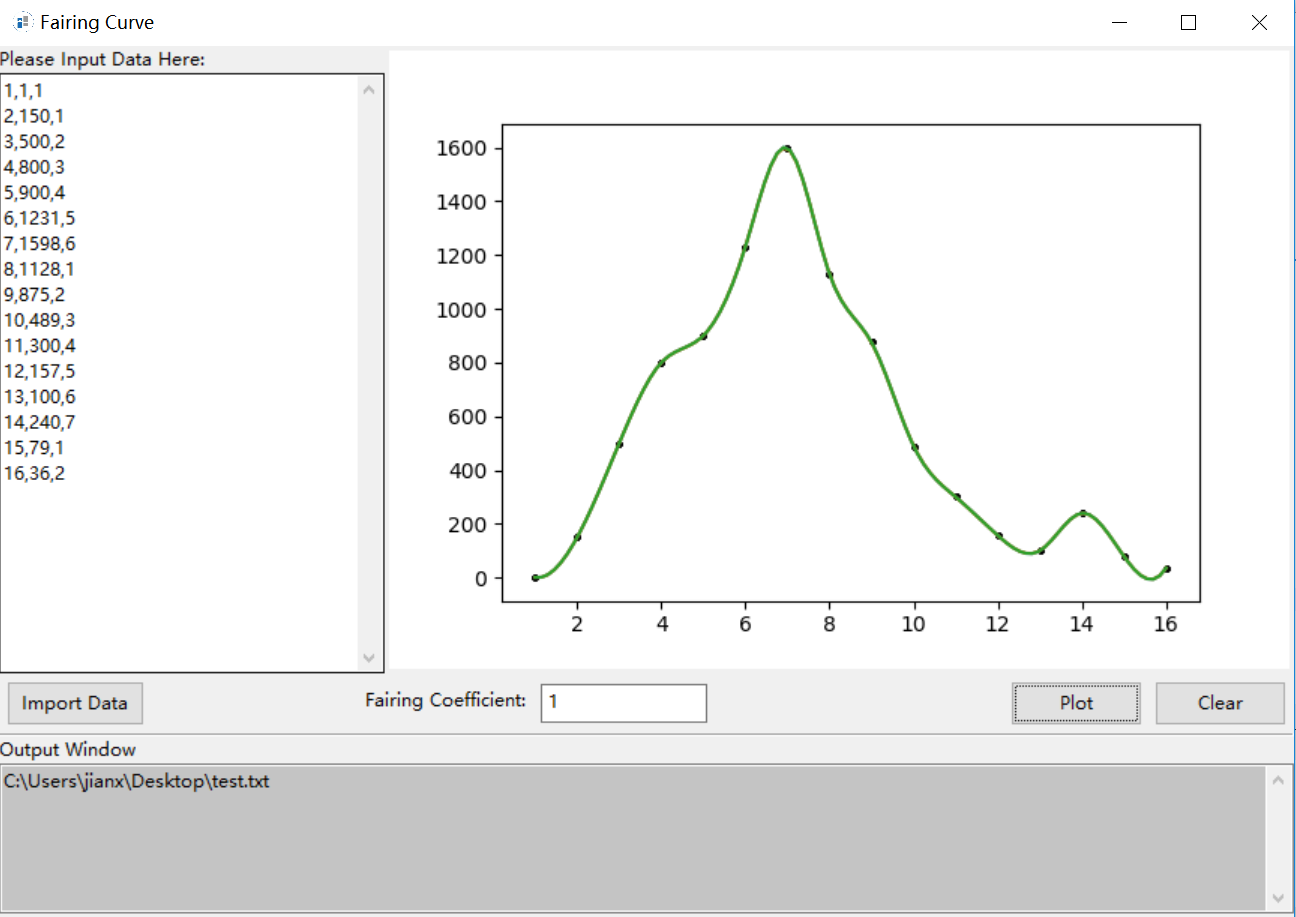
\includegraphics[width=4in]{weighted}
	\caption{An example with weight}
	\label{weighted}
\end{figure}
\end{document}